% Graphic for TeX using PGF
% Title: C:\Users\Kéké\Pictures\token.dia
% Creator: Dia v0.97.2
% CreationDate: Wed Feb 25 14:24:40 2015
% For: Kéké
% \usepackage{tikz}
% The following commands are not supported in PSTricks at present
% We define them conditionally, so when they are implemented,
% this pgf file will use them.
\ifx\du\undefined
  \newlength{\du}
\fi
\setlength{\du}{15\unitlength}
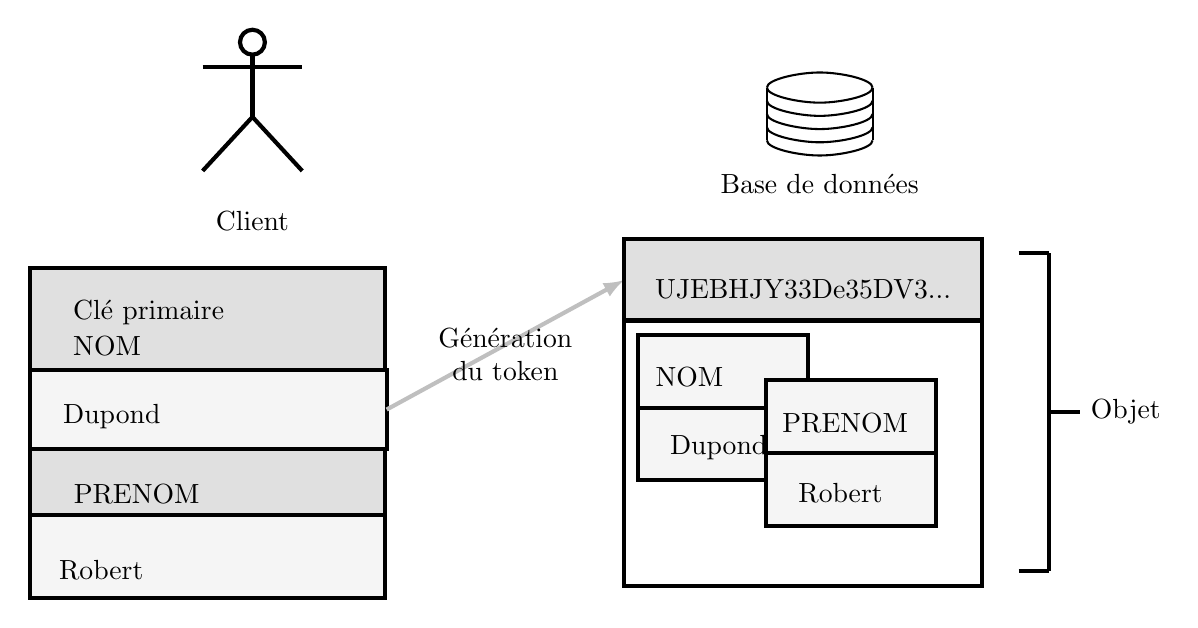
\begin{tikzpicture}
\pgftransformxscale{1.000000}
\pgftransformyscale{-1.000000}
\definecolor{dialinecolor}{rgb}{0.000000, 0.000000, 0.000000}
\pgfsetstrokecolor{dialinecolor}
\definecolor{dialinecolor}{rgb}{1.000000, 1.000000, 1.000000}
\pgfsetfillcolor{dialinecolor}
\pgfsetlinewidth{0.100000\du}
\pgfsetdash{}{0pt}
\pgfsetdash{}{0pt}
\pgfsetmiterjoin
\definecolor{dialinecolor}{rgb}{0.878431, 0.878431, 0.878431}
\pgfsetfillcolor{dialinecolor}
\fill (1.276183\du,5.800000\du)--(1.276183\du,8.250000\du)--(9.834956\du,8.250000\du)--(9.834956\du,5.800000\du)--cycle;
\definecolor{dialinecolor}{rgb}{0.000000, 0.000000, 0.000000}
\pgfsetstrokecolor{dialinecolor}
\draw (1.276183\du,5.800000\du)--(1.276183\du,8.250000\du)--(9.834956\du,8.250000\du)--(9.834956\du,5.800000\du)--cycle;
% setfont left to latex
\definecolor{dialinecolor}{rgb}{0.000000, 0.000000, 0.000000}
\pgfsetstrokecolor{dialinecolor}
\node[anchor=west] at (2.051183\du,6.875000\du){Clé primaire};
% setfont left to latex
\definecolor{dialinecolor}{rgb}{0.000000, 0.000000, 0.000000}
\pgfsetstrokecolor{dialinecolor}
\node[anchor=west] at (2.051183\du,7.675000\du){NOM};
\pgfsetlinewidth{0.100000\du}
\pgfsetdash{}{0pt}
\pgfsetdash{}{0pt}
\pgfsetmiterjoin
\definecolor{dialinecolor}{rgb}{0.960784, 0.960784, 0.960784}
\pgfsetfillcolor{dialinecolor}
\fill (1.280022\du,8.261125\du)--(1.280022\du,10.152994\du)--(9.873511\du,10.152994\du)--(9.873511\du,8.261125\du)--cycle;
\definecolor{dialinecolor}{rgb}{0.000000, 0.000000, 0.000000}
\pgfsetstrokecolor{dialinecolor}
\draw (1.280022\du,8.261125\du)--(1.280022\du,10.152994\du)--(9.873511\du,10.152994\du)--(9.873511\du,8.261125\du)--cycle;
% setfont left to latex
\definecolor{dialinecolor}{rgb}{0.000000, 0.000000, 0.000000}
\pgfsetstrokecolor{dialinecolor}
\node[anchor=west] at (1.808633\du,9.381975\du){Dupond};
\pgfsetlinewidth{0.100000\du}
\pgfsetdash{}{0pt}
\pgfsetdash{}{0pt}
\pgfsetmiterjoin
\definecolor{dialinecolor}{rgb}{0.878431, 0.878431, 0.878431}
\pgfsetfillcolor{dialinecolor}
\fill (1.275543\du,10.159437\du)--(1.275543\du,12.609437\du)--(9.834956\du,12.609437\du)--(9.834956\du,10.159437\du)--cycle;
\definecolor{dialinecolor}{rgb}{0.000000, 0.000000, 0.000000}
\pgfsetstrokecolor{dialinecolor}
\draw (1.275543\du,10.159437\du)--(1.275543\du,12.609437\du)--(9.834956\du,12.609437\du)--(9.834956\du,10.159437\du)--cycle;
% setfont left to latex
\definecolor{dialinecolor}{rgb}{0.000000, 0.000000, 0.000000}
\pgfsetstrokecolor{dialinecolor}
\node[anchor=west] at (2.063469\du,11.234437\du){PRENOM};
\pgfsetlinewidth{0.100000\du}
\pgfsetdash{}{0pt}
\pgfsetdash{}{0pt}
\pgfsetmiterjoin
\definecolor{dialinecolor}{rgb}{0.960784, 0.960784, 0.960784}
\pgfsetfillcolor{dialinecolor}
\fill (1.275543\du,11.752023\du)--(1.275543\du,13.745906\du)--(9.834956\du,13.745906\du)--(9.834956\du,11.752023\du)--cycle;
\definecolor{dialinecolor}{rgb}{0.000000, 0.000000, 0.000000}
\pgfsetstrokecolor{dialinecolor}
\draw (1.275543\du,11.752023\du)--(1.275543\du,13.745906\du)--(9.834956\du,13.745906\du)--(9.834956\du,11.752023\du)--cycle;
% setfont left to latex
\definecolor{dialinecolor}{rgb}{0.000000, 0.000000, 0.000000}
\pgfsetstrokecolor{dialinecolor}
\node[anchor=west] at (1.710227\du,13.076783\du){Robert};
\pgfsetlinewidth{0.100000\du}
\pgfsetdash{}{0pt}
\definecolor{dialinecolor}{rgb}{1.000000, 1.000000, 1.000000}
\pgfsetfillcolor{dialinecolor}
\pgfpathellipse{\pgfpoint{6.640293\du}{0.357590\du}}{\pgfpoint{0.300000\du}{0\du}}{\pgfpoint{0\du}{0.300000\du}}
\pgfusepath{fill}
\definecolor{dialinecolor}{rgb}{0.000000, 0.000000, 0.000000}
\pgfsetstrokecolor{dialinecolor}
\pgfpathellipse{\pgfpoint{6.640293\du}{0.357590\du}}{\pgfpoint{0.300000\du}{0\du}}{\pgfpoint{0\du}{0.300000\du}}
\pgfusepath{stroke}
\definecolor{dialinecolor}{rgb}{0.000000, 0.000000, 0.000000}
\pgfsetstrokecolor{dialinecolor}
\draw (5.440293\du,0.957590\du)--(7.840293\du,0.957590\du);
\definecolor{dialinecolor}{rgb}{0.000000, 0.000000, 0.000000}
\pgfsetstrokecolor{dialinecolor}
\draw (6.640293\du,0.657590\du)--(6.640293\du,2.157590\du);
\definecolor{dialinecolor}{rgb}{0.000000, 0.000000, 0.000000}
\pgfsetstrokecolor{dialinecolor}
\draw (6.640293\du,2.157590\du)--(5.440293\du,3.457590\du);
\definecolor{dialinecolor}{rgb}{0.000000, 0.000000, 0.000000}
\pgfsetstrokecolor{dialinecolor}
\draw (6.640293\du,2.157590\du)--(7.840293\du,3.457590\du);
% setfont left to latex
\definecolor{dialinecolor}{rgb}{0.000000, 0.000000, 0.000000}
\pgfsetstrokecolor{dialinecolor}
\node at (6.640293\du,4.652590\du){Client};
\pgfsetlinewidth{0.100000\du}
\pgfsetdash{}{0pt}
\pgfsetdash{}{0pt}
\pgfsetbuttcap
\pgfsetmiterjoin
\pgfsetlinewidth{0.100000\du}
\pgfsetbuttcap
\pgfsetmiterjoin
\pgfsetdash{}{0pt}
\definecolor{dialinecolor}{rgb}{1.000000, 1.000000, 1.000000}
\pgfsetfillcolor{dialinecolor}
\fill (19.033221\du,1.450486\du)--(19.033221\du,2.723213\du)--(21.578675\du,2.723213\du)--(21.578675\du,1.450486\du)--cycle;
\pgfsetbuttcap
\pgfsetmiterjoin
\pgfsetdash{}{0pt}
\definecolor{dialinecolor}{rgb}{1.000000, 1.000000, 1.000000}
\pgfsetfillcolor{dialinecolor}
\pgfpathellipse{\pgfpoint{20.305948\du}{2.723213\du}}{\pgfpoint{1.272727\du}{0\du}}{\pgfpoint{0\du}{0.363636\du}}
\pgfusepath{fill}
\pgfsetbuttcap
\pgfsetmiterjoin
\pgfsetdash{}{0pt}
\definecolor{dialinecolor}{rgb}{1.000000, 1.000000, 1.000000}
\pgfsetfillcolor{dialinecolor}
\pgfpathellipse{\pgfpoint{20.305948\du}{1.450486\du}}{\pgfpoint{1.272727\du}{0\du}}{\pgfpoint{0\du}{0.363636\du}}
\pgfusepath{fill}
\pgfsetlinewidth{0.050000\du}
\pgfsetbuttcap
\pgfsetmiterjoin
\pgfsetdash{}{0pt}
\definecolor{dialinecolor}{rgb}{0.000000, 0.000000, 0.000000}
\pgfsetstrokecolor{dialinecolor}
\pgfpathmoveto{\pgfpoint{19.033221\du}{1.450486\du}}
\pgfpathlineto{\pgfpoint{19.033221\du}{2.723213\du}}
\pgfusepath{stroke}
\pgfsetbuttcap
\pgfsetmiterjoin
\pgfsetdash{}{0pt}
\definecolor{dialinecolor}{rgb}{0.000000, 0.000000, 0.000000}
\pgfsetstrokecolor{dialinecolor}
\pgfpathmoveto{\pgfpoint{21.578675\du}{1.450486\du}}
\pgfpathlineto{\pgfpoint{21.578675\du}{2.723213\du}}
\pgfusepath{stroke}
\pgfsetbuttcap
\pgfsetmiterjoin
\pgfsetdash{}{0pt}
\definecolor{dialinecolor}{rgb}{0.000000, 0.000000, 0.000000}
\pgfsetstrokecolor{dialinecolor}
\pgfpathmoveto{\pgfpoint{19.033221\du}{1.450486\du}}
\pgfpathcurveto{\pgfpoint{19.033221\du}{1.249658\du}}{\pgfpoint{19.803875\du}{1.086849\du}}{\pgfpoint{20.305948\du}{1.086849\du}}
\pgfpathcurveto{\pgfpoint{20.808021\du}{1.086849\du}}{\pgfpoint{21.578675\du}{1.249658\du}}{\pgfpoint{21.578675\du}{1.450486\du}}
\pgfusepath{stroke}
\pgfsetbuttcap
\pgfsetmiterjoin
\pgfsetdash{}{0pt}
\definecolor{dialinecolor}{rgb}{0.000000, 0.000000, 0.000000}
\pgfsetstrokecolor{dialinecolor}
\pgfpathmoveto{\pgfpoint{19.033221\du}{1.450486\du}}
\pgfpathcurveto{\pgfpoint{19.033221\du}{1.651313\du}}{\pgfpoint{19.803875\du}{1.814122\du}}{\pgfpoint{20.305948\du}{1.814122\du}}
\pgfpathcurveto{\pgfpoint{20.808021\du}{1.814122\du}}{\pgfpoint{21.578675\du}{1.651313\du}}{\pgfpoint{21.578675\du}{1.450486\du}}
\pgfusepath{stroke}
\pgfsetbuttcap
\pgfsetmiterjoin
\pgfsetdash{}{0pt}
\definecolor{dialinecolor}{rgb}{0.000000, 0.000000, 0.000000}
\pgfsetstrokecolor{dialinecolor}
\pgfpathmoveto{\pgfpoint{19.033221\du}{1.768667\du}}
\pgfpathcurveto{\pgfpoint{19.033221\du}{1.969495\du}}{\pgfpoint{19.803875\du}{2.132304\du}}{\pgfpoint{20.305948\du}{2.132304\du}}
\pgfpathcurveto{\pgfpoint{20.808021\du}{2.132304\du}}{\pgfpoint{21.578675\du}{1.969495\du}}{\pgfpoint{21.578675\du}{1.768667\du}}
\pgfusepath{stroke}
\pgfsetbuttcap
\pgfsetmiterjoin
\pgfsetdash{}{0pt}
\definecolor{dialinecolor}{rgb}{0.000000, 0.000000, 0.000000}
\pgfsetstrokecolor{dialinecolor}
\pgfpathmoveto{\pgfpoint{19.033221\du}{2.086849\du}}
\pgfpathcurveto{\pgfpoint{19.033221\du}{2.287677\du}}{\pgfpoint{19.803875\du}{2.450486\du}}{\pgfpoint{20.305948\du}{2.450486\du}}
\pgfpathcurveto{\pgfpoint{20.808021\du}{2.450486\du}}{\pgfpoint{21.578675\du}{2.287677\du}}{\pgfpoint{21.578675\du}{2.086849\du}}
\pgfusepath{stroke}
\pgfsetbuttcap
\pgfsetmiterjoin
\pgfsetdash{}{0pt}
\definecolor{dialinecolor}{rgb}{0.000000, 0.000000, 0.000000}
\pgfsetstrokecolor{dialinecolor}
\pgfpathmoveto{\pgfpoint{19.033221\du}{2.405031\du}}
\pgfpathcurveto{\pgfpoint{19.033221\du}{2.605858\du}}{\pgfpoint{19.803875\du}{2.768667\du}}{\pgfpoint{20.305948\du}{2.768667\du}}
\pgfpathcurveto{\pgfpoint{20.808021\du}{2.768667\du}}{\pgfpoint{21.578675\du}{2.605858\du}}{\pgfpoint{21.578675\du}{2.405031\du}}
\pgfusepath{stroke}
\pgfsetbuttcap
\pgfsetmiterjoin
\pgfsetdash{}{0pt}
\definecolor{dialinecolor}{rgb}{0.000000, 0.000000, 0.000000}
\pgfsetstrokecolor{dialinecolor}
\pgfpathmoveto{\pgfpoint{19.033221\du}{2.723213\du}}
\pgfpathcurveto{\pgfpoint{19.033221\du}{2.924040\du}}{\pgfpoint{19.803875\du}{3.086849\du}}{\pgfpoint{20.305948\du}{3.086849\du}}
\pgfpathcurveto{\pgfpoint{20.808021\du}{3.086849\du}}{\pgfpoint{21.578675\du}{2.924040\du}}{\pgfpoint{21.578675\du}{2.723213\du}}
\pgfusepath{stroke}
% setfont left to latex
\definecolor{dialinecolor}{rgb}{0.000000, 0.000000, 0.000000}
\pgfsetstrokecolor{dialinecolor}
\node at (20.305948\du,3.777758\du){Base de données};
\pgfsetlinewidth{0.100000\du}
\pgfsetdash{}{0pt}
\pgfsetdash{}{0pt}
\pgfsetbuttcap
{
\definecolor{dialinecolor}{rgb}{0.749020, 0.749020, 0.749020}
\pgfsetfillcolor{dialinecolor}
% was here!!!
\pgfsetarrowsend{latex}
\definecolor{dialinecolor}{rgb}{0.749020, 0.749020, 0.749020}
\pgfsetstrokecolor{dialinecolor}
\draw (9.873511\du,9.207059\du)--(15.590683\du,6.088295\du);
}
% setfont left to latex
\definecolor{dialinecolor}{rgb}{0.000000, 0.000000, 0.000000}
\pgfsetstrokecolor{dialinecolor}
\node at (12.732097\du,7.470177\du){Génération};
% setfont left to latex
\definecolor{dialinecolor}{rgb}{0.000000, 0.000000, 0.000000}
\pgfsetstrokecolor{dialinecolor}
\node at (12.732097\du,8.270177\du){du token};
\pgfsetlinewidth{0.100000\du}
\pgfsetdash{}{0pt}
\pgfsetdash{}{0pt}
\pgfsetmiterjoin
\definecolor{dialinecolor}{rgb}{0.878431, 0.878431, 0.878431}
\pgfsetfillcolor{dialinecolor}
\fill (15.590683\du,5.098359\du)--(15.590683\du,7.078230\du)--(24.217262\du,7.078230\du)--(24.217262\du,5.098359\du)--cycle;
\definecolor{dialinecolor}{rgb}{0.000000, 0.000000, 0.000000}
\pgfsetstrokecolor{dialinecolor}
\draw (15.590683\du,5.098359\du)--(15.590683\du,7.078230\du)--(24.217262\du,7.078230\du)--(24.217262\du,5.098359\du)--cycle;
% setfont left to latex
\definecolor{dialinecolor}{rgb}{0.000000, 0.000000, 0.000000}
\pgfsetstrokecolor{dialinecolor}
\node at (19.903972\du,6.310795\du){UJEBHJY33De35DV3...};
\pgfsetlinewidth{0.100000\du}
\pgfsetdash{}{0pt}
\pgfsetdash{}{0pt}
\pgfsetmiterjoin
\definecolor{dialinecolor}{rgb}{1.000000, 1.000000, 1.000000}
\pgfsetfillcolor{dialinecolor}
\fill (15.590683\du,7.060556\du)--(15.590683\du,13.458267\du)--(24.217263\du,13.458267\du)--(24.217263\du,7.060556\du)--cycle;
\definecolor{dialinecolor}{rgb}{0.000000, 0.000000, 0.000000}
\pgfsetstrokecolor{dialinecolor}
\draw (15.590683\du,7.060556\du)--(15.590683\du,13.458267\du)--(24.217263\du,13.458267\du)--(24.217263\du,7.060556\du)--cycle;
\pgfsetlinewidth{0.100000\du}
\pgfsetdash{}{0pt}
\pgfsetdash{}{0pt}
\pgfsetmiterjoin
\definecolor{dialinecolor}{rgb}{0.960784, 0.960784, 0.960784}
\pgfsetfillcolor{dialinecolor}
\fill (15.926592\du,7.405185\du)--(15.926592\du,10.913659\du)--(20.013387\du,10.913659\du)--(20.013387\du,7.405185\du)--cycle;
\definecolor{dialinecolor}{rgb}{0.000000, 0.000000, 0.000000}
\pgfsetstrokecolor{dialinecolor}
\draw (15.926592\du,7.405185\du)--(15.926592\du,10.913659\du)--(20.013387\du,10.913659\du)--(20.013387\du,7.405185\du)--cycle;
\pgfsetlinewidth{0.100000\du}
\pgfsetdash{}{0pt}
\pgfsetdash{}{0pt}
\pgfsetbuttcap
{
\definecolor{dialinecolor}{rgb}{0.000000, 0.000000, 0.000000}
\pgfsetfillcolor{dialinecolor}
% was here!!!
\definecolor{dialinecolor}{rgb}{0.000000, 0.000000, 0.000000}
\pgfsetstrokecolor{dialinecolor}
\draw (15.926592\du,9.159422\du)--(20.013387\du,9.159422\du);
}
% setfont left to latex
\definecolor{dialinecolor}{rgb}{0.000000, 0.000000, 0.000000}
\pgfsetstrokecolor{dialinecolor}
\node[anchor=west] at (16.080811\du,8.426883\du){NOM};
% setfont left to latex
\definecolor{dialinecolor}{rgb}{0.000000, 0.000000, 0.000000}
\pgfsetstrokecolor{dialinecolor}
\node[anchor=west] at (16.427803\du,10.123288\du){Dupond};
\pgfsetlinewidth{0.100000\du}
\pgfsetdash{}{0pt}
\pgfsetdash{}{0pt}
\pgfsetmiterjoin
\definecolor{dialinecolor}{rgb}{0.960784, 0.960784, 0.960784}
\pgfsetfillcolor{dialinecolor}
\fill (19.018555\du,8.500016\du)--(19.018555\du,12.008490\du)--(23.105349\du,12.008490\du)--(23.105349\du,8.500016\du)--cycle;
\definecolor{dialinecolor}{rgb}{0.000000, 0.000000, 0.000000}
\pgfsetstrokecolor{dialinecolor}
\draw (19.018555\du,8.500016\du)--(19.018555\du,12.008490\du)--(23.105349\du,12.008490\du)--(23.105349\du,8.500016\du)--cycle;
\pgfsetlinewidth{0.100000\du}
\pgfsetdash{}{0pt}
\pgfsetdash{}{0pt}
\pgfsetbuttcap
{
\definecolor{dialinecolor}{rgb}{0.000000, 0.000000, 0.000000}
\pgfsetfillcolor{dialinecolor}
% was here!!!
\definecolor{dialinecolor}{rgb}{0.000000, 0.000000, 0.000000}
\pgfsetstrokecolor{dialinecolor}
\draw (19.018555\du,10.254253\du)--(23.105349\du,10.254253\du);
}
% setfont left to latex
\definecolor{dialinecolor}{rgb}{0.000000, 0.000000, 0.000000}
\pgfsetstrokecolor{dialinecolor}
\node[anchor=west] at (19.134219\du,9.521715\du){PRENOM};
% setfont left to latex
\definecolor{dialinecolor}{rgb}{0.000000, 0.000000, 0.000000}
\pgfsetstrokecolor{dialinecolor}
\node[anchor=west] at (19.519766\du,11.218120\du){Robert};
\pgfsetlinewidth{0.100000\du}
\pgfsetdash{}{0pt}
\pgfsetdash{}{0pt}
\pgfsetbuttcap
\pgfsetmiterjoin
\pgfsetlinewidth{0.100000\du}
\pgfsetbuttcap
\pgfsetmiterjoin
\pgfsetdash{}{0pt}
\definecolor{dialinecolor}{rgb}{0.000000, 0.000000, 0.000000}
\pgfsetstrokecolor{dialinecolor}
\draw (25.098715\du,13.103743\du)--(25.831254\du,13.103743\du);
\pgfsetbuttcap
\pgfsetmiterjoin
\pgfsetdash{}{0pt}
\definecolor{dialinecolor}{rgb}{0.000000, 0.000000, 0.000000}
\pgfsetstrokecolor{dialinecolor}
\draw (25.098715\du,5.431365\du)--(25.831254\du,5.431365\du);
\pgfsetbuttcap
\pgfsetmiterjoin
\pgfsetdash{}{0pt}
\definecolor{dialinecolor}{rgb}{0.000000, 0.000000, 0.000000}
\pgfsetstrokecolor{dialinecolor}
\draw (25.831254\du,13.103743\du)--(25.831254\du,5.431365\du);
\pgfsetbuttcap
\pgfsetmiterjoin
\pgfsetdash{}{0pt}
\definecolor{dialinecolor}{rgb}{0.000000, 0.000000, 0.000000}
\pgfsetstrokecolor{dialinecolor}
\draw (26.563793\du,9.267554\du)--(25.831254\du,9.267554\du);
% setfont left to latex
\definecolor{dialinecolor}{rgb}{0.000000, 0.000000, 0.000000}
\pgfsetstrokecolor{dialinecolor}
\node at (22.901100\du,9.467554\du){};
% setfont left to latex
\definecolor{dialinecolor}{rgb}{0.000000, 0.000000, 0.000000}
\pgfsetstrokecolor{dialinecolor}
\node[anchor=west] at (26.563793\du,9.267554\du){Objet};
\end{tikzpicture}
